\documentclass[11pt,a4paper]{report}

\usepackage[top=25mm,bottom=25mm,right=25mm,left=30mm,head=12.5mm,foot=12.5mm]{geometry}
%\let\openright=\cleardoublepage

\usepackage[a-2u]{pdfx}

\usepackage[
   backend=biber
%  ,style=iso-authoryear
  ,style=alphabetic
  ,citestyle=numeric
  ,sortlocale=cs_CZ
  ,bibencoding=UTF8
  %,block=ragged
]{biblatex}
\addbibresource{references.bib}

%% Přepneme na českou sazbu, fonty Latin Modern a kódování češtiny
\usepackage[czech]{babel}
\usepackage{lmodern}
\usepackage[T1]{fontenc}
\usepackage{textcomp}
\usepackage[utf8]{inputenc}

% Set fonts
\RequirePackage[osf]{mathpazo} % Palatino with oldstyle figures
\newcommand\liningnums[1]{\fontfamily{ppl}\selectfont#1}
\RequirePackage{eulervm}
\RequirePackage[scaled=.8819]{sourcecodepro} % Source Code Pro typeface for monospace

%%% Další užitečné balíčky (jsou součástí běžných distribucí LaTeXu)
\usepackage{amsmath}        % rozšíření pro sazbu matematiky
\usepackage{amsfonts}       % matematické fonty
\usepackage{amsthm}         % sazba vět, definic apod.
\usepackage{bm}             % tučné symboly (příkaz \bm)
\usepackage{graphicx}       % vkládání obrázků
\usepackage{fancyvrb}       % vylepšené prostředí pro strojové písmo
\usepackage{fancyhdr}       % prostředí pohodlnější nastavení hlavy a paty stránek
\usepackage{icomma}         % inteligetní čárka v matematickém módu
\usepackage{dcolumn}        % lepší zarovnání sloupců v tabulkách
\usepackage{booktabs}       % lepší vodorovné linky v tabulkách
\makeatletter
\@ifpackageloaded{xcolor}{
   \@ifpackagewith{xcolor}{usenames}{}{\PassOptionsToPackage{usenames}{xcolor}}
  }{\usepackage[usenames]{xcolor}} % barevná sazba
\makeatother
\usepackage{multicol}       % práce s více sloupci na stránce
\usepackage{caption}
\usepackage{enumitem}
\usepackage{lipsum}
\setlist[itemize]{noitemsep, topsep=0pt, partopsep=0pt}
\setlist[enumerate]{noitemsep, topsep=0pt, partopsep=0pt}
\setlist[description]{noitemsep, topsep=0pt, partopsep=0pt}
\usepackage{pdfpages}

\usepackage{tocloft}
\setlength\cftparskip{0pt}
\setlength\cftbeforechapskip{1.5ex}
\setlength\cftfigindent{0pt}
\setlength\cfttabindent{0pt}
\setlength\cftbeforeloftitleskip{0pt}
\setlength\cftbeforelottitleskip{0pt}
\setlength\cftbeforetoctitleskip{0pt}
\renewcommand{\cftlottitlefont}{\Huge\bfseries}
\renewcommand{\cftloftitlefont}{\Huge\bfseries}
\renewcommand{\cfttoctitlefont}{\Huge\bfseries}

%Barevná syntaxe kódu
\usepackage{listings}
\renewcommand{\lstlistlistingname}{Seznam kódů}% Listing -> Seznam kódů
\definecolor{bluekeywords}{rgb}{0,0,1}
\definecolor{greencomments}{rgb}{0,0.5,0}
\definecolor{redstrings}{rgb}{0.64,0.08,0.08}
\definecolor{xmlcomments}{rgb}{0.5,0.5,0.5}
\definecolor{types}{rgb}{0.17,0.57,0.68}
\lstset{language=[Sharp]C,
captionpos=b,
numbers=left,
frame=lines,
showspaces=false,
showtabs=false,
breaklines=true,
showstringspaces=false,
breakatwhitespace=true,
escapeinside={(*@}{@*)},
commentstyle=\color{greencomments},
morekeywords={partial, var, value, get, set},
keywordstyle=\color{bluekeywords},
stringstyle=\color{redstrings},
basicstyle=\ttfamily\small,
numbers=left, 
}
% vyznaceni odstavcu
\parindent=0pt
\parskip=11pt

% zakaz vdov a sirotku - jednoradkovych pocatku ci koncu odstavcu na prechodu mezi strankami
\clubpenalty=1000
\widowpenalty=1000
\displaywidowpenalty=1000

% nastaveni radkovani
\renewcommand{\baselinestretch}{1.20}

% nastavení hlavy a paty stránek
\fancyhf{}
%\renewcommand{\chaptermark}[1]{\markboth{#1}{}}
%\fancyhead[L]{\leftmark}
\fancyhead[C]{\AutorPrace, \Kruh}
\fancyfoot[R]{\thepage}
\fancyhead[L]{ÚPA semestrální práce}
\fancyhead[R]{\today}
%\renewcommand{\footrulewidth}{0pt}
%\fancypagestyle{plain}{%
%\fancyhf{} % clear all header and footer fields
%\fancyfoot[R]{\thepage}
%\renewcommand{\headrulewidth}{0pt}
%\renewcommand{\footrulewidth}{0.5pt}
%}
\fancypagestyle{plain}{
\fancyhead[C]{\AutorPrace, \Kruh}
\fancyhead[R]{\today}
\fancyfoot[R]{\thepage}
\fancyhead[L]{ÚPA semestrální práce}
}

% Tato makra přesvědčují mírně ošklivým trikem LaTeX, aby hlavičky kapitol
% sázel příčetněji a nevynechával nad nimi spoustu místa. Směle ignorujte.
\makeatletter
\def\@makechapterhead#1{
  {\parindent \z@ \raggedright 
   \Huge\bfseries \thechapter. #1
   \par\nobreak
   \vskip 20\p@
}}
\def\@makeschapterhead#1{
  {\parindent \z@ \raggedright 
   \Huge\bfseries #1
   \par\nobreak
   \vskip 20\p@
}}
\makeatother

% Trochu volnější nastavení dělení slov, než je default.
\lefthyphenmin=2
\righthyphenmin=2

% Zapne černé "slimáky" na koncích řádků, které přetekly, abychom si
% jich lépe všimli.
\overfullrule=1mm

%% Balíček hyperref, kterým jdou vyrábět klikací odkazy v PDF,
%% ale hlavně ho používáme k uložení metadat do PDF (včetně obsahu).
%% Většinu nastavítek přednastaví balíček pdfx.
\hypersetup{unicode}
\hypersetup{breaklinks=true}
\hypersetup{hidelinks}

%%% Prostředí pro sazbu kódu, případně vstupu/výstupu počítačových
%%% programů. (Vyžaduje balíček fancyvrb -- fancy verbatim.)

\DefineVerbatimEnvironment{code}{Verbatim}{fontsize=\small, frame=single}



\def\NazevPrace{Určení hodnoty Ludolfova čísla pomocí řady, kterou navrhl James Gregory}
\def\Kruh{159}
\def\AutorPrace{Vladislav Aulich}
\def\DatumOdevzdani{2021}

% Vedoucí práce: Jméno a příjmení s~tituly
\def\Vedouci{Ing. Jan Kohout}

% Fakulta a obor
\def\StudijniProgram{Fyzikální a výpočetní chemie}
\def\Fakulta{Fakulta chemicko-inženýrská}

\begin{document}
	
	%%% Titulní strana práce a další povinné informační strany

%%% Titulní strana práce

\pagestyle{empty}
\pagenumbering{gobble}
\hypersetup{pageanchor=false}

\begin{center}

\vspace{\stretch{8}}


\includegraphics[width=.8\textwidth]{img/logo}

\vspace{\stretch{8}}

{\Huge\bfseries\NazevPrace}

\vspace{8mm}
\mdseries{Semestrální práce}

\vspace{\stretch{8}}
\large
\begin{tabular}{rl}
Autor: & \AutorPrace \\
\noalign{\vspace{2mm}}
Kruh: & \Kruh\\
\noalign{\vspace{2mm}}
Studijní obor: & \StudijniProgram\\
\noalign{\vspace{2mm}}
Fakulta: & \Fakulta\\
\noalign{\vspace{2mm}}
Akademický rok: & 2021/2022\\
\noalign{\vspace{2mm}}
Předmět: & Úvod do programování a algoritmů \\
\noalign{\vspace{2mm}}
Vedoucí práce: & \Vedouci \\
\end{tabular}

\vspace{20mm}
Praha, \DatumOdevzdani
\end{center}

\pagenumbering{arabic}
	
	% Obsah
	\setcounter{tocdepth}{2}
	\tableofcontents
	
	\chapter{Teoretická část}
	\pagestyle{fancy}
		
	\section{Zadání úlohy}
	Určete hodnotu Ludolfova čísla pomocí řady, kterou navrhl James Gregory.
	
	\section{Úvod}
	Snahy o~stanovení hodnoty čísla $\pi$ sahají hluboko do historie. Jednou z~mnoha možností je vyjádření Ludolfova čísla pomocí Maclaurinova rozvoje funkce $\arctan(x)$. Za objevitele této řady bývá považován skotský matematik James Gregory, který ji objevil v~polovině 17.století. Nezávisle na Gregorym dospěl k~stejné řadě také  Gottfried W. 
    Leibniz, proto také bývá někdy označována jako Leibnizova nebo Gregory-Leibniz řada.
    
    $$\arctan(x) = x-\frac{x^3}{3}+\frac{x^5}{5}-\frac{x^7}{7}+\frac{x^9}{9}...$$
    
    Dosazením $x = 1$ získáme funkční hodnotu funkce $\arctan(1)=\frac{\pi}{4}$. Pokud tyto úpravy provedeme pro celou řadu, získáme pro aproximaci čísla $\pi$ následující vztah:
    $$\frac{\pi}{4}=1-\frac{1}{3}+\frac{1}{5}-\frac{1}{7}...$$
    $$\pi=4\left(1-\frac{1}{3}+\frac{1}{5}-\frac{1}{7}...\right)$$
    
    Tato řada konverguje ke skutečné hodnotě čísla $\pi$ velmi pomalu, pro určení čísla s~přesností na dvě desetinná místa musíme provést téměř 300 iterací\footnote{\url{https://web.archive.org/web/20071128201346/http://www.scm.org.co/Articulos/832.pdf}}. Tato vlastnost je je citelná zejména pro ruční výpočty, které musel Gregory provádět.
    
    Z~této řady vychází další myšlenky pro stanovení čísla $\pi$. Zrychlení konvergence řady navrhl Abraham Sharp, který dosadil hodnotu $x=\sqrt{\frac{1}{3}}$. Tímto způsobem následně získal hodnotu čísla na 72 platných cifer.
	

	\chapter{Implementace}
	\section{Postup řešení}
	Pro součet této řady byla vytvořena metoda nazvaná VypocitejPi. Vstupní parametr je počet iterací (členů řady), pro které se má stanovit hodnota $\pi$. Parametr je datového typu uint, protože se jedná o~celé kladné číslo. Návratovou hodnotou je stanovený výsledek čísla $\pi$ datového typu decimal.
	
	V~metodě je využito pomocné proměnné \uv{pomocna}, která zaznamenává hodnotu zlomku (člena řady). Následně je v~programu rozhodovací logika, která buď hodotu zlomku přičte nebo odečte od hodnoty proměnné \uv{soucet}. V~proměnné součet je uložena aproximovaná hodnota $\pi$, která se s každou iterací přibližuje té skutečné.
	
	Dále je v~programu ošetřován uživatelův vstup \uv{n}, který označuje počet iterací. Ten byl zadáním omezen na 10 000 000, stejně jako zaokrouhlení výstupu na 8 desetinných míst. Hodnotu 10 000 000 jsem zvolil z důvodu pomalé konvergence řady. V~programu je dále použitá pomocná proměnná \uv{pokracovat}, slouží k~opakování načtení vstupu v~případě špatně zadaného vstupu (do-while cyklus).
	
	\subsection{Časová složitost algoritmu}
	Program obsahuje pouze jeden for cyklus, který se provádí n krát v~závislosti na délce uživatelova vstupu. Algoritmus tedy spadá do časové složitosti $\mathcal{O}(n)$.
	
	\section{Použitý software}
	Pro tvorbu dokumentace bylo využito prostředí online \LaTeX editoru Overleaf. Jako podklad byla využita šablona k~maturitní práci Gymnázia Jana Keplera, která byla graficky upravena.
	
	Programování samotné aplikace probíhalo ve vývojovém prostředí Visual Studio 2017 od společnosti Microsoft. Změny na projektu byly průběžně zaznamenávány verzovacím systémem Git a následně vkládány na server Github. Odkaz na repozitář: \url{https://github.com/aulichv/pi_Gregory.git}.
	
	\clearpage
	\section{Zdrojový kód}
        \begin{lstlisting}[caption=Výsledný zdrojový kód]
        using System;
        using System.Collections.Generic;
        using System.Linq;
        using System.Text;
        using System.Threading.Tasks;
        
        namespace semestralka_konsole
        {
            class Program
            {
                /// <summary>
                /// Metoda, ktera pomoci rady Jamese Gregoryho
                /// stanovy hodnotu Ludolfova cisla.
                /// </summary>
                /// <param name="n">Pocet iteraci (clenu rady)</param>
                /// <returns>Hodnota pi datoveho typu decimal</returns>
                public static decimal VypocitejPi(uint n)
                {
                    decimal soucet = 0;
                    decimal pomocna = 0;
                    for (int i = 0; i < n; i++)
                    {
        
                        pomocna = 4m / (1 + (2 * i));
                        //Pro sude koeficienty
                        if (i % 2 == 0)
                            soucet += pomocna;
                        //Pro liche koeficienty
                        else
                            soucet -= pomocna;
                    }
                    return soucet;
                }
                static void Main(string[] args)
                {
                    bool pokracovat = true;
                    uint n = 0;
                    decimal pi = 0;
                    do
                    {
                        Console.WriteLine("Zadejte pocet iteraci:");
                        try
                        {
                            n = uint.Parse(Console.ReadLine());
                            //Stanoveni podminky poctu opakovani
                            if (n > 10000000)
                            {
                                //Upozorni uzivatele na spatny vstup
                                Console.WriteLine("Zadejte prosim cele kladne cislo mensi nez 10 000 000");
                            }
                            else
                                //Spravna hodnota n, ukonci smycku a vypocte pi
                                pokracovat = false;
                        }
        
                        catch (Exception e)
                        {
                            Console.WriteLine("Zadejte prosim cele kladne cislo mensi nez 10 000 000");
                        }
                    }
                    while (pokracovat);
                    //Provedeni funkce pro uzivatelem zadany pocet iteraci a zaokrouhleni na 8 desetinnych mist
                    pi = Math.Round(VypocitejPi(n), 8);
                    Console.WriteLine("Hodnota Ludolfova cisla pro {0} iteraci je {1}", n, pi);
                    Console.WriteLine("Pro ukonceni programu stisknete libovolnou klavesu.");
                    Console.ReadKey();
                }
            }
        }

        \end{lstlisting}
	\section{Ukázka programu}
	\begin{figure}[h!]
			\centering
			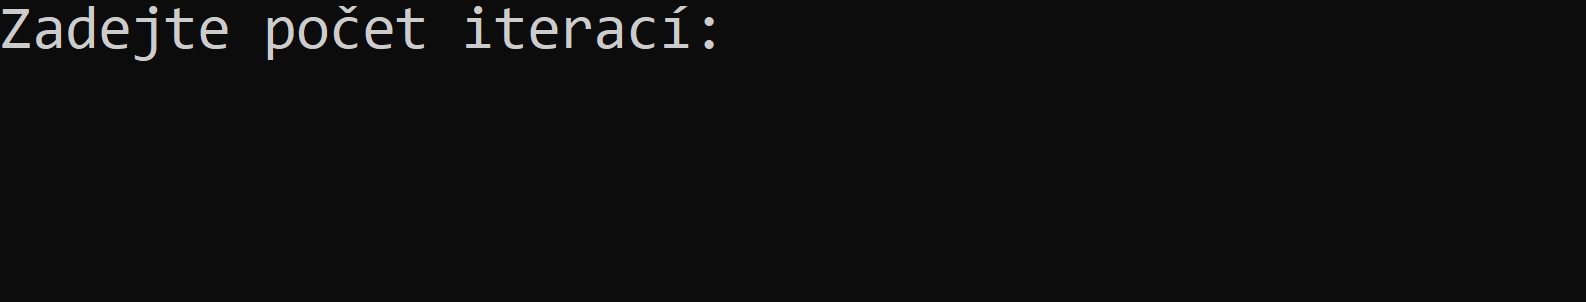
\includegraphics[width=0.7\hsize]{img/spusteni.png}
			\caption{Obrazovka po spuštění programu}
		\end{figure}
		
	\begin{figure}[]
			\centering
			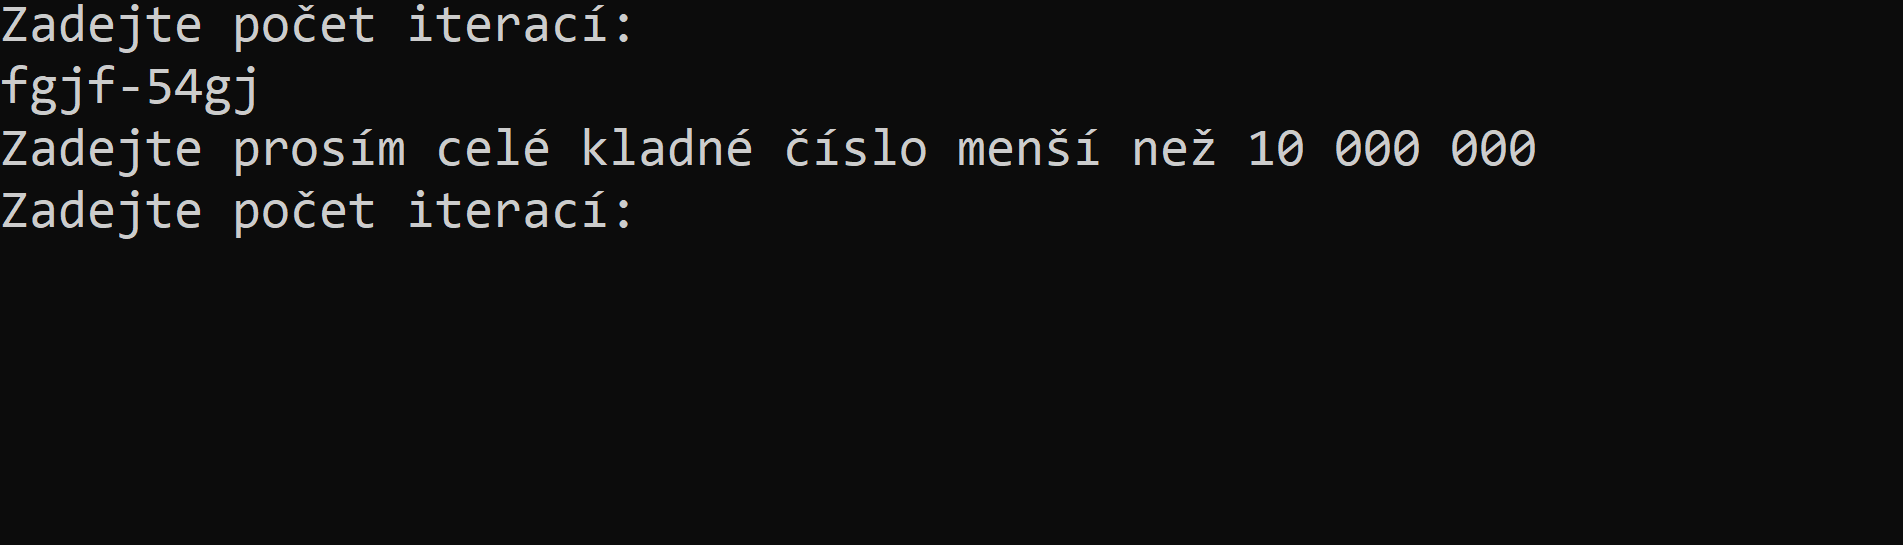
\includegraphics[width=1\hsize]{img/spusteni_chybny_vstup.png}
			\caption{Hláška programu při špatném uživatelském vstupu}
		\end{figure}
		
	\begin{figure}[]
			\centering
			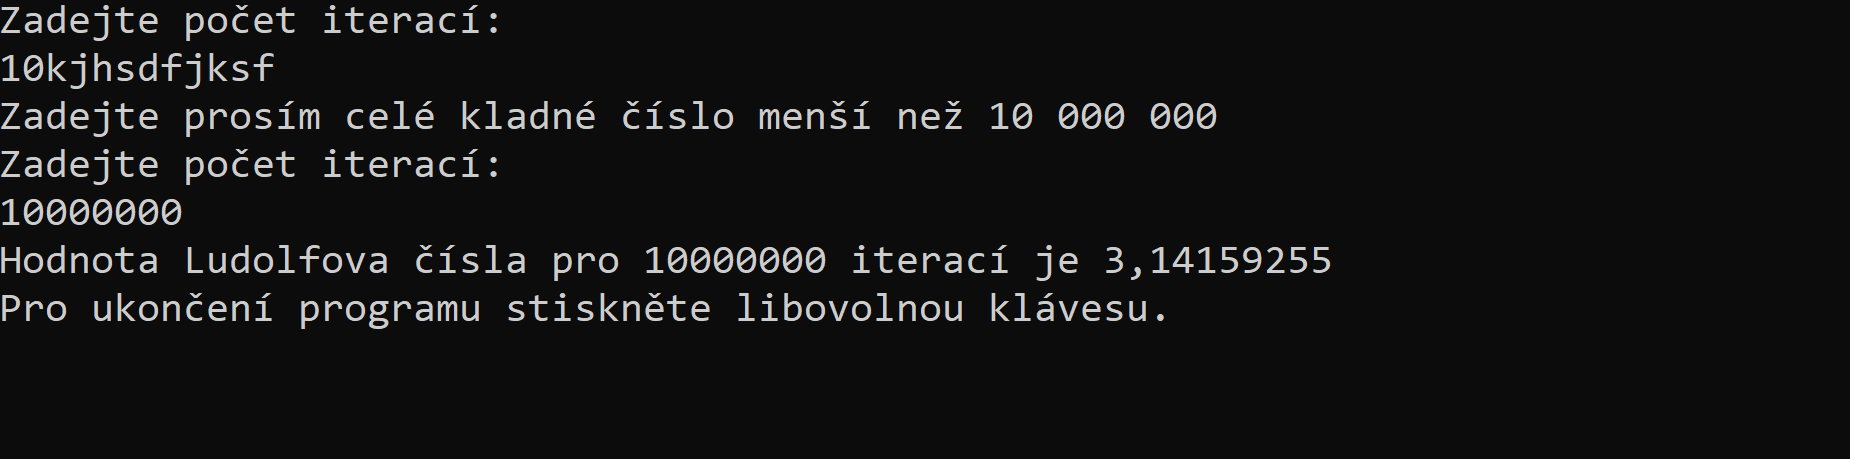
\includegraphics[width=1\hsize]{img/spusteni_vysledek.png}
			\caption{Výstup programu pro zadaný počet iterací}
		\end{figure}
	
	\chapter*{Závěr}
	\pagestyle{empty}
	\addcontentsline{toc}{chapter}{Závěr}
	Při práci na projektu jsem se dozvěděl mnoho zajímavostí o~historii čísla $\pi$. Zejména o~jeho významu v~matematice a snahách o~stanovení jeho hodnoty. 
	
	Dále jsem rozšířil své znalosti o~sázení zdrojového kódu v~sázecím jazyce \LaTeX. Původně jsem kód vykresloval pomocí balíčku \uv{verbatim}, u~toho se mi však nepovedlo nastavit kód podle mých představ. Nakonec jsem tedy použil balíček \uv{listings}. U~něj jsem narážel na problémy s~kódem obsahujícím diakritiku. Ten se mi vyřešit nepodařilo, vložený kód je tedy bez diakritiky.
	
	K~tvorbě dokumentace jsem využíval webový nástroj Overleaf a jednotlivé verze jsem verzoval v~repozitáři umístěném na serveru Github. Nové zkušenosti jsem získal i přizpůsobením si vývojového prostředí Visual Studio.
	
	Práci na projektu považuji za přínosnou a domnívám se, že jsem zadání splnil.

	%%% Seznam použité literatury
	\nocite{dokumentace}
	\nocite{medium}
	\nocite{citace}
	\nocite{Historie_pi}
	\nocite{wiki:pi}
	\nocite{zvyrazneni_kodu}
	\nocite{clisting}
	\nocite{aproximace_pi}
	\printbibliography[title={Seznam použité literatury},heading={bibintoc}]
	
	
    %%% Seznam obrázků
	\clearpage
	\listoffigures
	\addcontentsline{toc}{chapter}{Seznam obrázků}
	
	%%% Seznam tabulek
	\clearpage
	\lstlistoflistings

	
	%%% Přílohy k práci, existují-li. Každá příloha musí být alespoň jednou
	%%% odkazována z vlastního textu práce. Přílohy se číslují.
	
	%\part*{Přílohy}
	%\appendix
	
\end{document}
